% !TeX spellcheck = fr_FR

% TODO: Replace scan images with clean text where possible

\documentclass[a4paper, 10pt]{report}

\usepackage[french]{babel}
\usepackage[T1]{fontenc}

\usepackage{amsmath, amssymb, amsfonts}

\usepackage{hyperref}
\usepackage{geometry}

\usepackage{xcolor}
\usepackage{graphicx}

\usepackage{fancyhdr}
\usepackage{lastpage}

\usepackage{enumitem}

\geometry{
	a4paper,
	left=25mm,
	right=25mm,
	top=35mm,
	bottom=25mm,
	headsep=5mm,
	headheight=20mm,
}

\definecolor{solution}{HTML}{E5E4E2}
\providecommand{\abs}[1]{\lvert#1\rvert}
\providecommand{\norm}[1]{\lVert#1\rVert}
\DeclareMathOperator{\card}{card}

\begin{document}
	
	\renewcommand{\headrule}{%
		\vspace{-4pt}\hrulefill
		\raisebox{-6.8pt}{\ 
\includegraphics[height=5mm]{../../icon.png}}
		\hrulefill
	}	
	\pagestyle{fancy}
	\fancyhf{}
	
	\fancyhead[L]{\small \slshape Automne 2024}
	\fancyhead[C]{\Large \bfseries Analyse I - Série 07}
	\fancyhead[R]{\small Buff Mathias}
	\fancyfoot[L]{
		\small Source files available at:
		\href{https://github.com/MathiasBuff/bsc-math}
		{github.com/MathiasBuff/bsc-math}
	}
	\fancyfoot[R]{
		\small Page \thepage
		\hspace{1pt} /
		\pageref*{LastPage}
	}
	

	\noindent
	\textbf{Exercice 1.} Soient deux réels $a$ et $b$. Montrer que la
	fonction $x \mapsto ax + b$ est uniformément continue. Déterminer
	l'ensemble des $k > 0$ pour lesquels cette fonction est
	$k$-Lipschitzienne.
	
	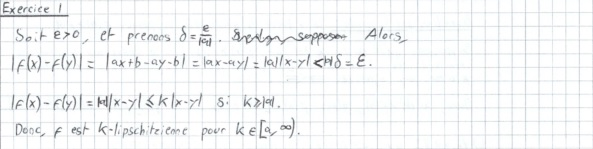
\includegraphics{ex01.jpg}
	
	\vspace{5mm}
	\noindent
	\textbf{Exercice 2.} (Fonctions $\alpha$-Hölderiennes)\\
	Soit $I$ un intervalle de $\mathbb{R}$ non nécessairement borné.
	Une fonction $f: I \to \mathbb{R}$ est $\alpha$-Hölderienne
	(où $\alpha > 0$) s'il existe $C > 0$ tel que pour tout $x, y \in I$,
	$\abs{f(x) - f(y)} \leq C \abs{x-y}^\alpha$.
	\begin{enumerate}[label=(\roman*)]
		\item Montrer qu'une fonction Hölderienne est uniformément
		continue.
		%
		\item Montrer que $x \mapsto \sqrt{x}$ est 1/2-Hölderienne sur
		$I = \mathbb{R}_+$. (En revanche, en classe nous avons montré que
		$x \mapsto \sqrt{x}$ n'est $k$-Lipschitzienne pour aucun $k$.)
		%
		\item Montrer qu'une fonction $\alpha$-Hölderienne est constante
		si $\alpha > 1$.
	\end{enumerate}
	
	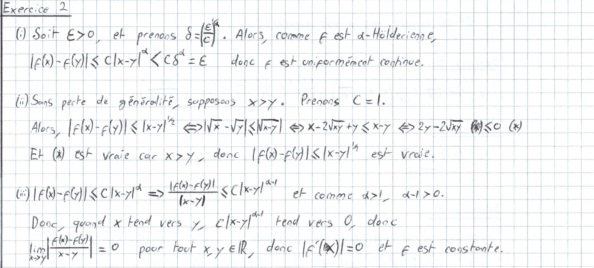
\includegraphics{ex02.jpg}
	
	\newpage
	
	\fancyhf{}
	\renewcommand{\headrule}
	{\rule{\textwidth}{0pt}}
	\fancyfoot[R]{
		\small Page \thepage
		\hspace{1pt} /
		\pageref*{LastPage}
	}
	
	\noindent
	\textbf{Exercice 3.} Soit $f: \mathbb{R} \to \mathbb{R}$ continue.
	Supposons que $f$ tend vers zéro en $+\infty$ et en $-\infty$.
	\begin{enumerate}[label=(\roman*)]
		\item Soit $\varepsilon > 0$, montrer qu'il existe $M > 0$ tel
		que pour tout $x \in \mathbb{R} \setminus [-M, M]$, on a
		$\abs{f(x)} < \varepsilon/2$. 
		%
		\item Montrer qu'il existe $\delta > 0$ tel que pour tout
		$x, y \in [-(M+1), M+1]$ tels que $\abs{x - y} < \delta$ on a
		$\abs{f(x) - f(y)} < \varepsilon$.
		%
		\item Déduire des deux questions précédentes que $f$ est
		uniformément continue sur $\mathbb{R}$.
		%
		\item Montrer que $f$ est bornée.
	\end{enumerate}
	
	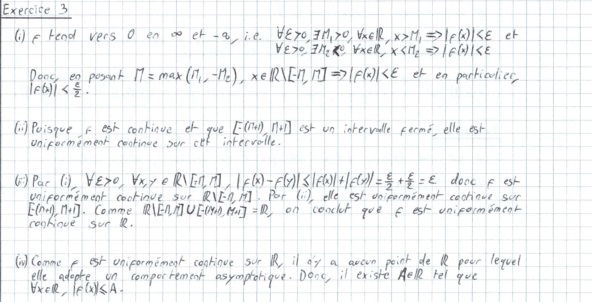
\includegraphics{ex03.jpg}
		
	\vspace{5mm}
	\noindent
	\textbf{Exercice 4.} soit $I$ un intervalle et $f \in C(I, \mathbb{R})$
	injective. Le but de cet exercice est de montrer que $f$ est monotone.
	\begin{enumerate}[label=(\roman*)]
		\item Soient $a < x < b$ dans $I$. Montrer que $f(x)$ est
		strictement comprise entre $f(a)$ et $f(b)$.\\
		(\textit{Indication :} théorème des valeurs intermédiaires.)
		%
		\item Conclure que $f$ est monotone.
	\end{enumerate}
	
	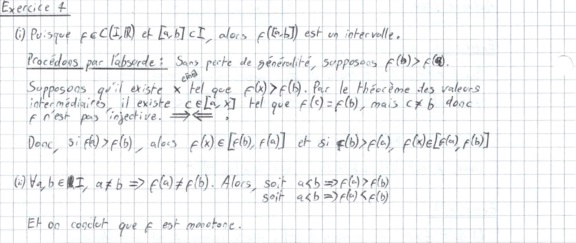
\includegraphics{ex04.jpg}
		
	\newpage
	
	\noindent
	\textbf{Exercice 5.} Calculer la dérivée de la fonction
	$f: \mathbb{R} \to \mathbb{R}^2$,
	\[f(x) = \left(x^3 - x, \frac{1}{x^2 + 1}\right)\]
	
	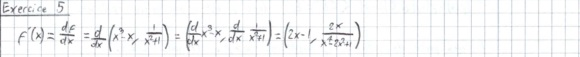
\includegraphics{ex05.jpg}
		
	\vspace{5mm}
	\noindent
	\textbf{Exercice 6.} Donner une fonction $f: (0, 1) \to \mathbb{R}$
	continue qui n'est pas uniformément continue.
	
	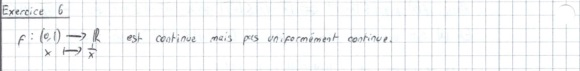
\includegraphics{ex06.jpg}
		
	\vspace{5mm}	
	\noindent
	\textbf{Exercice 7.} Soit $f: \mathbb{R} \to \mathbb{R}$ continue
	et \textit{périodique}, c'est-à-dire que $f(x+1) = f(x)$ pour
	tout $x \in \mathbb{R}$. Montrer que $f$ est bornée et
	uniformément continue.
	
	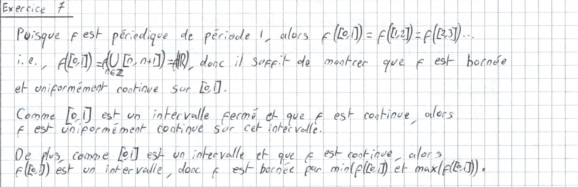
\includegraphics{ex07.jpg}
		
	\vspace{5mm}	
	\noindent
	\textbf{Exercice 8.} On définit $f: \mathbb{R} \to \mathbb{R}$ par
	la formule
	\[
		f(x) = \left\{\begin{aligned}
			&0\quad \text{ si $x$ est irrationnel,}\\
			&\tfrac{1}{q}\quad \text{ si $x$ est rationnel et s'écrit
				$x = \tfrac{p}{q}$ avec $p$ et $q$ premiers entre eux.}
		\end{aligned}\right.
	\]
	Montrer que $f$ est discontinue en tout point rationnel et continue
	en tout point irrationnel.
	
	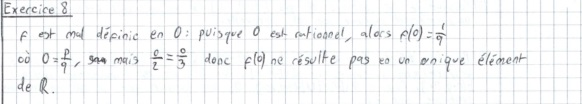
\includegraphics{ex08.jpg}
	
%	
%	
%	\colorbox{solution}
%	{
%		\begin{minipage}{0.9\textwidth}
%			s
%		\end{minipage}
%	}
%	
%	\colorbox{solution}
%	{
%		\begin{minipage}{0.9\textwidth}
%			\begin{enumerate}[label=(\alph*)]
%				\item a
%			\end{enumerate}
%		\end{minipage}
%	}
	
\end{document}
